\documentclass[12pt]{article}

\usepackage[english]{babel}
\usepackage{graphicx}
\usepackage[numbers]{natbib}
\usepackage{gitinfo2}
\usepackage{amsmath}
\usepackage[T1]{fontenc}
\usepackage[utf8]{inputenc}
\usepackage{authblk}
\usepackage{color,soul}
\usepackage{xcolor}
\usepackage{framed}
\usepackage{multirow}

\definecolor{Mycolor2}{HTML}{BBBBEE}
\definecolor{Mycolor3}{HTML}{EEBBBB}

\colorlet{shadecolor}{Mycolor2}
\DeclareRobustCommand{\hlb}[1]{{\sethlcolor{Mycolor2}\hl{#1}}}

\renewcommand\Authands{ and }
\newcommand\tab[1][1cm]{\hspace*{#1}}

\title{A simple statistical model describing burnt area through limitations on fire}

\author[2]{Bistinas, I}
\author[5, 6]{Burton, C}
\author[1]{Kelley, D \thanks{\textbf{Email:} douglas.i.kelley@gmail.com
                                   \textbf{Web}: douglask3.github.io}}
\author[1]{Marthews, T}
\author[3, 4]{Whitley, R}


\affil[1]{Centre for Ecology and Hydrology\\
          Maclean Building \\
          Crowmarsh Gifford \\
          Wallingford \\
          Oxfordshire \\
          United Kingdom}

\affil[2]{Vrije Universiteit Amsterdam\\
          Faculty of Earth and Life Sciences \\
          Amsterdam \\
          Netherlands}

\affil[3]{Suncorp Group \\
          Personal Lines Pricing Research \\
          Sydney \\
          Australia}

\affil[4]{Macquarie University \\
          Department of Biological Sciences \\
          Sydney \\
          Australia}

\affil[5]{Met Office UK \\
          Exeter \\
          UK}

\affil[6]{Geography \\
          University of Exeter \\
          Exeter \\
          UK}


\begin{document}
\maketitle

\begin{center}
    \textbf{git info}

        git url: https://github.com/douglask3/LimFIRE

	    git revision no: \gitAbbrevHash

        Last commit author: \gitAuthorName,  \gitAuthorEmail

	    Branch: \gitReferences

	    Revision Date: \gitAuthorIsoDate
\end{center}
\newpage

\begin{abstract}
    \textbf{Aim}
    Spatial and temporal patterns of burnt area are controlled by
        availability of fuel,
        fuel moisture,
        natural and anthropogenic ignitions,
        and anthropagenic suppression.
    Here, we map the limitation and sensitivity of burnt area to each of these controls.

    \textbf{Location}
    Global

    \textbf{Methods}
    We describe a simple framework whereby limitations are imposed by:
        fuel discontinuity;
        fuel moisture and atmospheric drying potential;
        lightning and human ignitions;
        and land use.
    Limitations are described from remote sensed and meteorological observations and optimized against Global Fire Emissions Database (GFED4s) burnt area observations.

    \textbf{Results}
    Fuel moisture is shown to be the main limitation of fire over much of the world, (44\% annual average and 36\% during local dry seasons), particularly in the humid forests and cold, slow drying boreal areas.
    Fuel discontinuity is the next limitation (25\% annually and 23\% in the dry season), especially in deserts and dry season grasslands.
    This is followed by land use change (18\% annually, 21\% dry season)
    and then ignitions (13\% annually, 19\% dry season), which is only a significant limiting factor in dry season savanna,
    where rapid drying of fuel built up during the wet season removes all other natural limitations. In these areas, changes in burnt area are actually more sensitive to other controls, typically land use.

    \textbf{Main conclusions}
    This study contradicts the way basic processes are represented in many global fire models.
    As ignitions only impact burnt area over a limited geographic extent, better representation of controls imposed by fuel loads and moisture is vital. Human ignitions only contribute to a small increase in global burnt area (2%), which is
    offset by the dramatic impact of suppression through anthropogenic land cover changes.
    The assumption
    that humans cause burnt area over much of the world is therefore clearly incorrect, and adequate simulation
    of suppression through land use should become a priority. This result also has implications when considering
    ecosystem services of agricultural land and fire management policies
\end{abstract}

%\section{Introduction}
\pgfdeclareimage[width=1.0\paperwidth]{header-image}{header_images/kata_tjuta}

\begin{frame}
    \frametitle{It burns where it rains}
    \framesubtitle{Unimodal relationship with moisture}

    \foreach \x in {1, 2, 3, 4, 5, 6, 7, 8, 9, 10, 11, 12} {
        \only<\x> {
        \begin{textblock*}{10cm}(0cm,1.5cm)
            \includegraphics[width=13.0cm]{images/unimodal/p\x.png}%images/unimodal/p\x.png}
    \end{textblock*}
    }}
    %Make clear we are talking about burnt area
\end{frame}

\begin{frame}<1-3>[label = intro]
    \frametitle{What else controls fire?}
    \framesubtitle{Is it Ignitions? Is it people?}
	\begin{itemize}
		\visible<2-> {\item Fire-vegetation models incorporate ignition schemes}
		\visible<3-> {\item Schemes often include human and lightning caused ignitions}
		\visible<4-> {\item All models with human-caused ignitions show increased burnt area with people}
		\visible<5-> {\item Little effort placed in anthropagenic fire suppression}
	\end{itemize}

\end{frame}

\begin{frame}
    \frametitle{What else controls fire?}
    \framesubtitle{Is it Ignitions? Is it people?}
    FireMIP slide from Stijn
    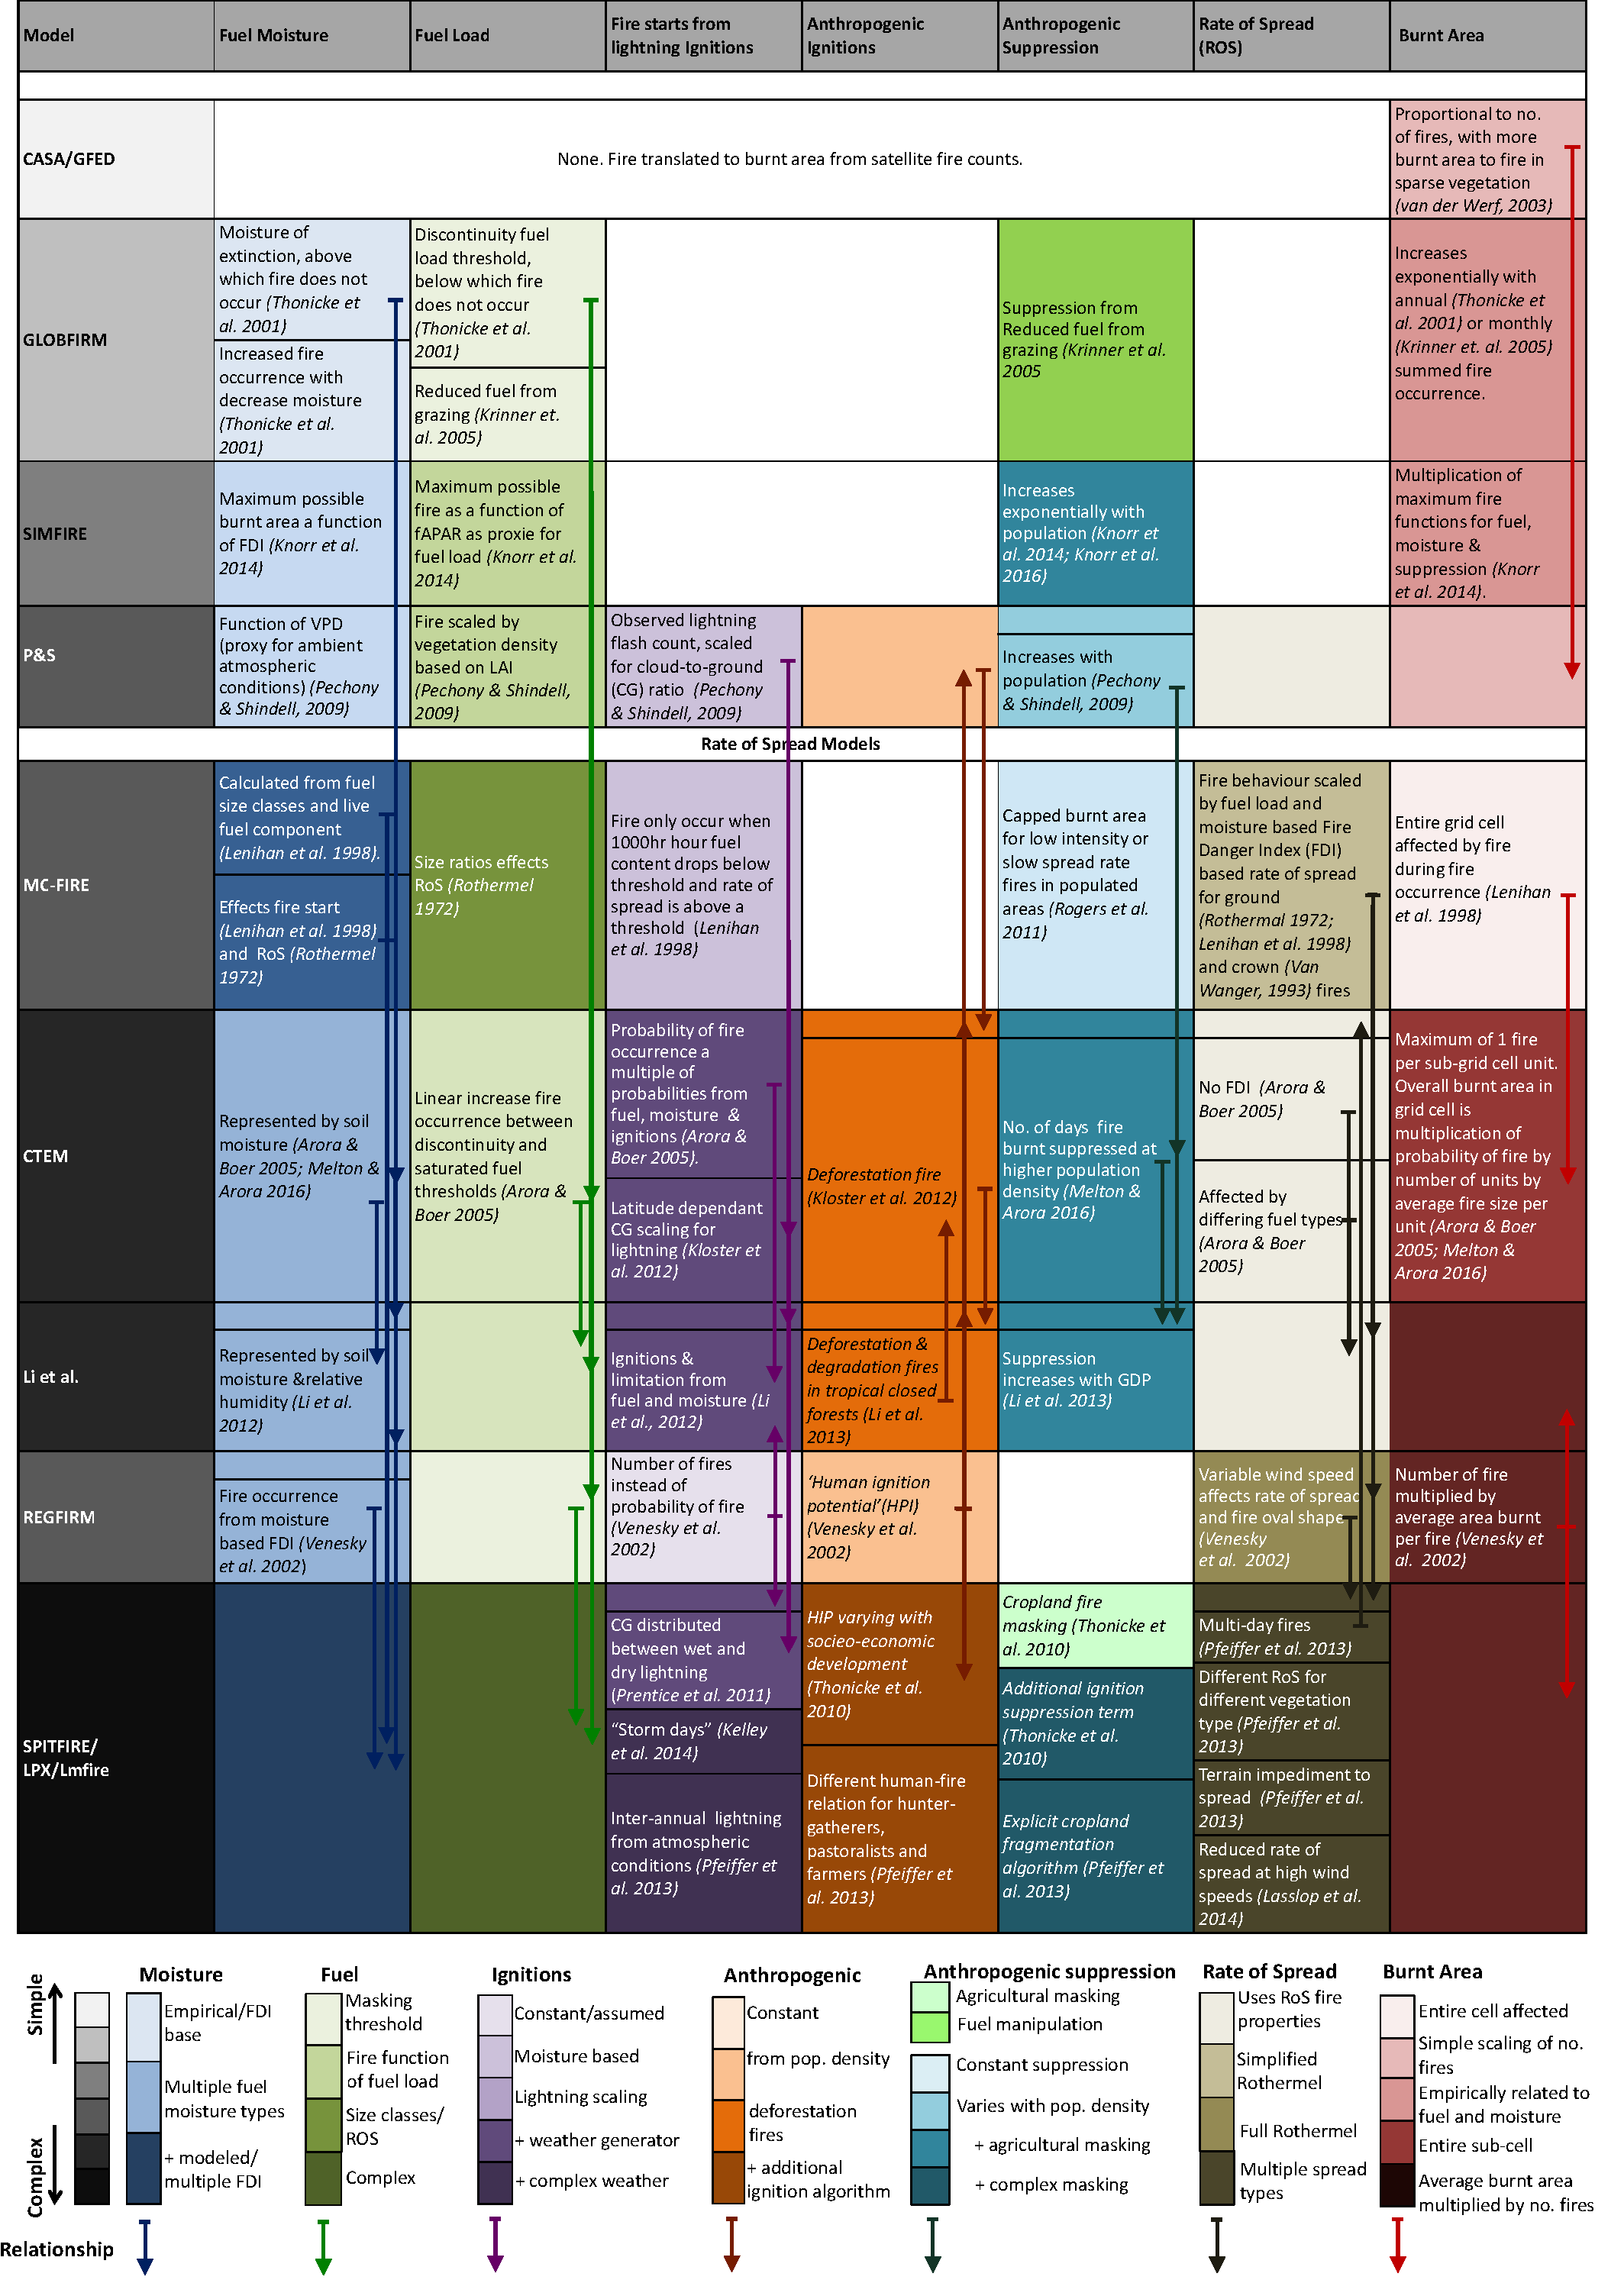
\includegraphics[width=3cm]{images/Table1.pdf}%images/unimodal/p\x.png}
\end{frame}

\againframe<3-4>{intro}

\begin{frame}
    \frametitle{What else controls fire?}
    \framesubtitle{Is it Ignitions? Is it people?}
    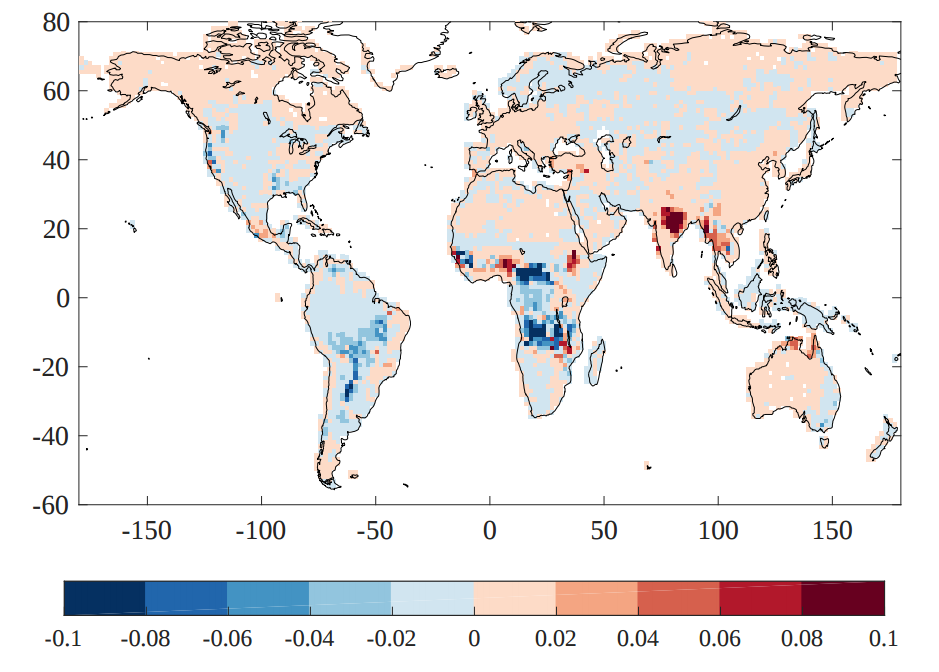
\includegraphics[width=9.0cm]{images/INFERNO}%images/unimodal/p\x.png}
	%Inferno plot
\end{frame}

\againframe<4->{intro}

\begin{frame}
    \frametitle{What else controls fire?}
    \framesubtitle{Fire-limitation framework}
	\begin{itemize}
		\visible<2-> {\item Map the limitation and sensitivity of burnt area to}
        \begin{itemize}
            \visible<3-> {\item Fuel discontinuity}
            \visible<4-> {\item Fuel moisture and atmospheric drying potential}
            \visible<5-> {\item lightning and human ignitions}
            \visible<6-> {\item land use and human suppression}
        \end{itemize}
		\visible<7-> {\item Controls are described from remote sensed and meteorological observations}
		\visible<8-> {\item optimized againstburnt area observations}
	\end{itemize}
\end{frame}

\section{Methods}
\pgfdeclareimage[width=1.0\paperwidth]{header-image}{header_images/Sierra_Calderona}

\def \inputMap#1#2#3#4 {
    \begin{backgroundblock}{#1}{#2}
        \begin{tikzpicture}
            \node[anchor=south west,inner sep=0] (image) at (0,0) {
                \includegraphics[width=4.0cm]{images/inputs/#3}
            };
            \node[align=center, font = {\tiny}] at (2.15cm, 2.33cm) {#4};
        \end{tikzpicture}
    \end{backgroundblock}
}

\def \inputMapA#1#2 {
    \inputMap{5cm}{1.33cm}{#1}{#2}
}
\def \inputMapB#1#2 {
    \inputMap{6.67cm}{3.67cm}{#1}{#2}
}
\def \inputMapC#1#2 {
    \inputMap{8.33cm}{6cm}{#1}{#2}
}

\begin{frame}<2-5>[label=framework]
    \frametitle{Fire limitation framework}
    \framesubtitle{Spatial and Temporal controls on burnt area}

    \begin{tikzpicture}
        \visible<2->{\fill[blue , opacity = 0.7] (90:4) -- (210:4) -- (-30:4) -- cycle;}
        \visible<3->{\fill[green,path fading=south, opacity = 0.85] (90:4) -- (210:4) -- (-30:4) -- cycle;}
        \visible<4->{\fill[red  ,path fading=west, opacity = 0.7] (90:4) -- (210:4) -- (-30:4) -- cycle;}

       
        \visible<2>{
            \node (note) at (0, 1.5em) {\Huge Moisture Content};
            \node (note) at (0, 0.0em) {\large Live Fuel};
            \node (note) at (0,-1.5em) {\large Atmosphere};
        }

        \visible<3->{
            \node[rotate = 30] at (-2.5, -1.3) {\large Moisture};
        }
    
	     \visible<3>{
	    	\node (note) at (0,1.5em) {\Huge Fuel Load};
	    	\node (note) at (0,0) {\large Net Primary Production};
	    }
	    
	   % \visible<4->{
	   % 	\node[rotate = -30] at (2.6,-1.3) {\large Fuel};
	    %	\node[rotate = -30] at (2.4,-1.6) {NPP};
	   % }	
    
	    \visible<4->{
	    	\node[anchor = east, rotate = 90] at (0, 3.3) {\large Fuel};
	    }
    
        \visible<4>{
            \node (note) at (0,1.5em) {\Huge Ignitions};
            \node (note) at (0,0) { \large Lightning};
            \node (note) at (0,-1.25em) { \large Population Density};
            \node (note) at (0,-2.5em) { \large Pasture};
        }

        \visible<5->{
           \node[rotate = -30] at (2.5, -1.3) {\large Ignitions};
        }

        \visible<5>{
            \node (note) at (0,0) {\Huge Burnt Area};
        }

    \end{tikzpicture}

    \begin{textblock*}{5cm}(6.67cm,2cm)
        \visible<7->{
            \begin{tikzpicture}[scale=0.67]
                \fill[green] (90:4) -- (210:4) -- (-30:4) -- cycle;
                \fill[blue,path fading=west] (90:4) -- (210:4) -- (-30:4) -- cycle;
                \fill[red,path fading=south] (90:4) -- (210:4) -- (-30:4) -- cycle;
                \fill[black, opacity = 0.3] (90:4) -- (210:4) -- (-30:4) -- cycle;
            \end{tikzpicture}
        }
    \end{textblock*}

    \begin{textblock*}{5cm}(10.1cm,2cm)
        \visible<7->{
            \begin{tikzpicture}[scale=0.33]
                \fill[green] (90:4) -- (210:4) -- (-30:4) -- cycle;
                \fill[blue,path fading=west] (90:4) -- (210:4) -- (-30:4) -- cycle;
                \fill[red,path fading=south] (90:4) -- (210:4) -- (-30:4) -- cycle;
                \fill[black, opacity = 0.5] (90:4) -- (210:4) -- (-30:4) -- cycle;
            \end{tikzpicture}
        }
    \end{textblock*}

    \begin{textblock*}{4.5cm}(4.6cm,2.6cm)
        \visible<7->{
            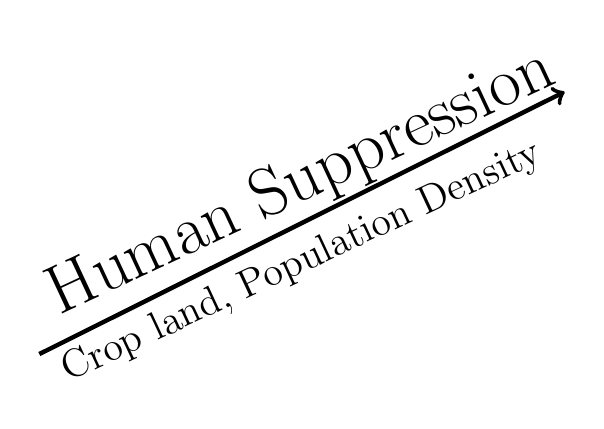
\begin{tikzpicture}
                \node[rotate = 25 ] (note) at (3.335, 2.165) {\Huge Human Suppression};
                    \node[rotate = 25 ] (note) at (3.335, 1.165) {\Large Crop land, Population Density};
                \draw[ultra thick, ->] (0, 0) -- (6.67, 3.33);
            \end{tikzpicture}
        }
    \end{textblock*}

	\only<2> {
		\inputMap{5cm}{1.18cm}{inputs_mean-alpha}{STASH $\frac{Actual}{Potential}$ Evapotranspiration \\ (Whitley et al 2014; Davis et al 2016)}
		\inputMapB{inputs_mean-emc}{Equilibrium Fuel Moisture Content}
	}


    \only<3> {
        \inputMapA{inputs_mean-npp}{MODIS NPP (MODIS 17)}
    }

    \only<4> {
        \inputMapA{inputs_mean-Lightn}{LIS/OTD (Christian 1999)}
        \inputMapB{inputs_mean-popdens}{HYDE Popdens (Goldewijk  et al 2011)}
        \inputMapC{inputs_mean-pas}{HYDE Pasture (Goldewijk et al 2011)}
    }

	\only<7> {
		\inputMap{4.7cm}{1.33cm}{inputs_mean-popdens}{HYDE Popdens (Goldewijk et al 2011)}
		\inputMap{8.33cm}{6cm}{inputs_mean-crop}{HYDE crop (Goldewijk et al 2011)}
	}

    \only<5> {
    	\begin{backgroundblock}{4.2cm}{1.33cm}
    		\begin{tikzpicture}
		         \node[anchor=south west,inner sep=0] (image) at (0,0) {
		        	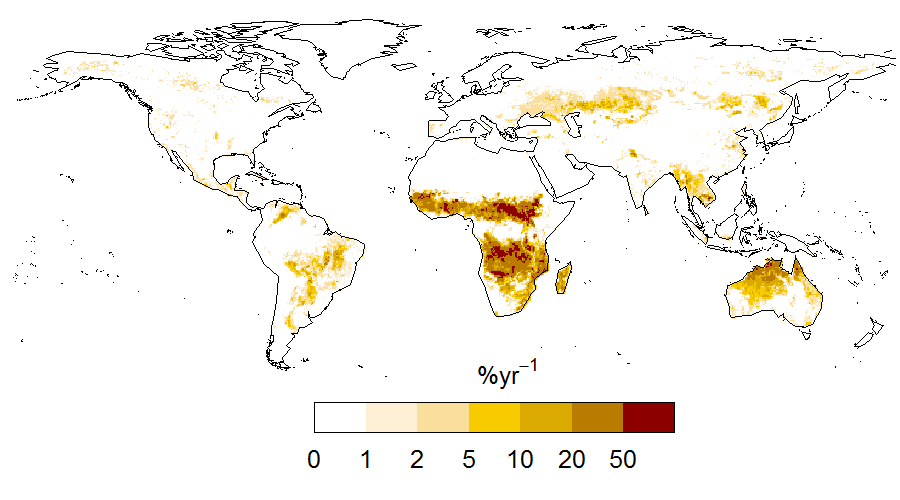
\includegraphics[width=7.0cm]{images/inputs/inputs_mean-fire}
		        };
		        \node[align=center, font = {\small}] at (2.95cm, 4.2cm) {Global Fire Emission Database 4s \\ (Giglio et al 2013; Randerson et al 2012)};
	        \end{tikzpicture}
	    \end{backgroundblock}
        %?% Make bigger
    }
    %?% Stuff to include:
    %?%   Monthly -> Inter annual and seasonal controls
\end{frame}

\def \controlsSide#1 {
    \begin{textblock*}{11cm}(0cm,1.5cm)
        \begin{tikzpicture}
            \node[anchor=south west,inner sep=0] (image) at (0,0) {
                \includegraphics[width=13.0cm]{images/#1}
            };
            \visible<-4> {\draw[white, fill = white] (6.5,3.0) -- (13.0,3.0) -- (13.0,7) -- (6.5,7) -- (6.5,3.0);}
            \visible<-1> {\draw[white, fill = white] (0.0,0.0) -- ( 6.5,0.0) -- ( 6.5,3.5) -- (0.0,3.5) -- (0.0,0.0);}
           \visible<-4>  {\draw[white, fill = white] (6.5,3.0) -- (13.0,3.0) -- (13.0,0.0) -- (6.5,0.0) -- (6.5,3.0);}
            %\visible<-4> {\draw[white, fill = white] (0.0,0) -- (12.0,0) -- (12.0,1.0) -- (0.0,1.0) -- (0.0,0);}
        \end{tikzpicture}
    \end{textblock*}
    \begin{textblock*}{11cm}(2.0cm, 7.5cm)
        \includegraphics[width=5.0cm]{images/#1_legend}
    \end{textblock*}
}

\pgfdeclareimage[width=1.0\paperwidth]{header-image}{header_images/kata_tjuta}

\begin{frame}
	\frametitle{Controls on fire}
	%\framesubtitle{Geographic controls}
	\begin{textblock*}{14cm}(0.3cm,1.2cm)
		\includegraphics[width=5.78cm]{images/limitCurves/NPPVsFire}	
	\end{textblock*}
	\begin{textblock*}{14cm}(6.5cm,1.2cm)
		\includegraphics[width=5.78cm]{images/limitCurves/alphaVsFire}	
	\end{textblock*}
	\begin{textblock*}{14cm}(0.32cm,5cm)
		\includegraphics[width=5.78cm]{images/limitCurves/ignitionsVsFire.png}		
	\end{textblock*}
	\begin{textblock*}{14cm}(6.5cm,5.3cm)
		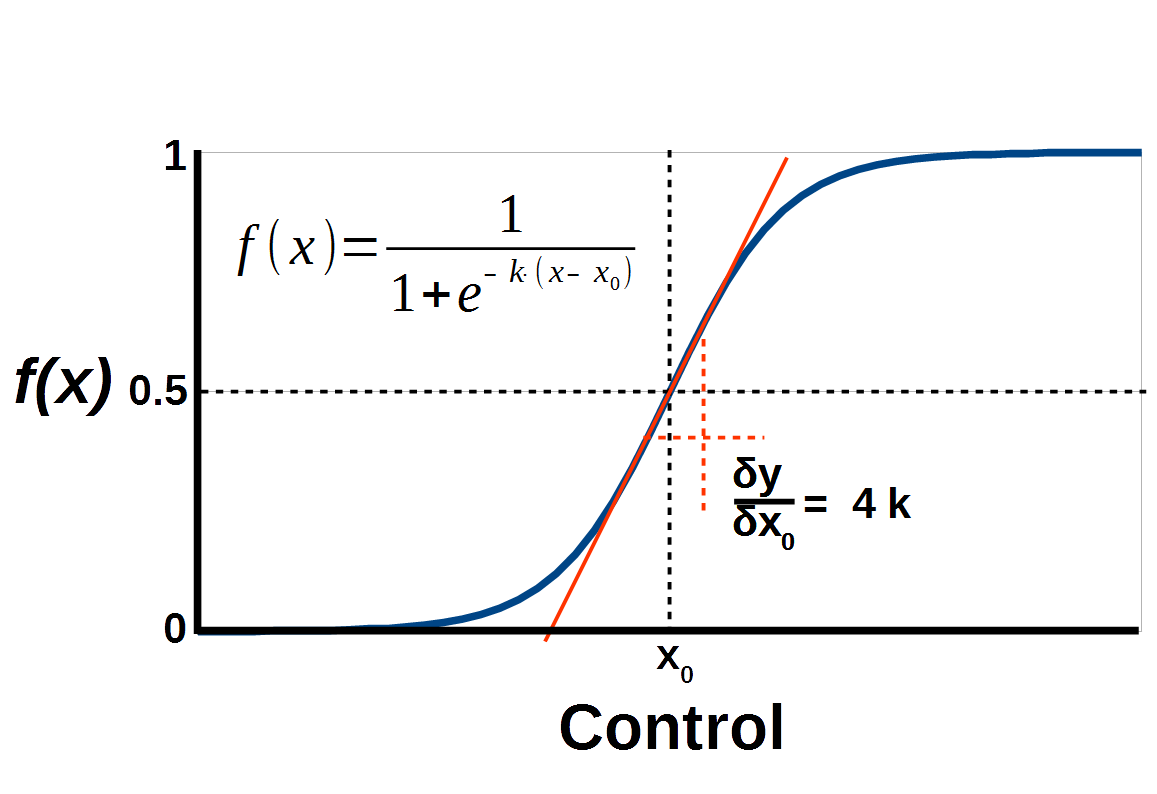
\includegraphics[width=5.78cm]{../diagrams/Logistic_fun.png}		
	\end{textblock*}
\end{frame}
\addtocounter{framenumber}{-1}

\begin{frame}
	\frametitle{Controls on fire}
	%\framesubtitle{Geographic controls}
	\begin{textblock*}{14cm}(0.3cm,1.2cm)
		\includegraphics[width=5.78cm]{images/limitCurves/NPPVsFire}	
	\end{textblock*}
	\begin{textblock*}{14cm}(6.5cm,1.2cm)
		\includegraphics[width=5.78cm]{images/limitCurves/alphaVsFire}	
	\end{textblock*}
	\begin{textblock*}{14cm}(0.32cm,5cm)
		\includegraphics[width=5.78cm]{images/limitCurves/ignitionsVsFire.png}		
	\end{textblock*}
	\begin{textblock*}{14cm}(6.5cm,5.3cm)
		\includegraphics[width=5.78cm]{images/limitCurves/fireMap.png}		
	\end{textblock*}
\end{frame}
\addtocounter{framenumber}{-1}

\begin{frame}
	\frametitle{Controls on fire}
	%\framesubtitle{Geographic controls}
	\begin{textblock*}{14cm}(0.3cm,1.2cm)
		\includegraphics[width=5.78cm]{images/limitCurves/Desert/NPPVsFire}	
	\end{textblock*}
	\begin{textblock*}{14cm}(6.5cm,1.2cm)
		\includegraphics[width=5.78cm]{images/limitCurves/Desert/alphaVsFire}	
	\end{textblock*}
	\begin{textblock*}{14cm}(0.32cm,5cm)
		\includegraphics[width=5.78cm]{images/limitCurves/Desert/ignitionsVsFire.png}		
	\end{textblock*}
	\begin{textblock*}{14cm}(6.5cm,5.3cm)
		\includegraphics[width=5.78cm]{images/limitCurves/Desert/fireMap.png}		
	\end{textblock*}
\end{frame}
\addtocounter{framenumber}{-1}

\begin{frame}
	\frametitle{Controls on fire}
	%\framesubtitle{Geographic controls}
	\begin{textblock*}{14cm}(0.3cm,1.2cm)
		\includegraphics[width=5.78cm]{images/limitCurves/RainF/NPPVsFire}	
	\end{textblock*}
	\begin{textblock*}{14cm}(6.5cm,1.2cm)
		\includegraphics[width=5.78cm]{images/limitCurves/RainF/alphaVsFire}	
	\end{textblock*}
	\begin{textblock*}{14cm}(0.32cm,5cm)
		\includegraphics[width=5.78cm]{images/limitCurves/RainF/ignitionsVsFire.png}		
	\end{textblock*}
	\begin{textblock*}{14cm}(6.5cm,5.3cm)
		\includegraphics[width=5.78cm]{images/limitCurves/RainF/fireMap.png}		
	\end{textblock*}
\end{frame}
\addtocounter{framenumber}{-1}

\begin{frame}
	\frametitle{Controls on fire}
	%\framesubtitle{Geographic controls}
	\begin{textblock*}{14cm}(0.3cm,1.2cm)
		\includegraphics[width=5.78cm]{images/limitCurves/Savanna/NPPVsFire}	
	\end{textblock*}
	\begin{textblock*}{14cm}(6.5cm,1.2cm)
		\includegraphics[width=5.78cm]{images/limitCurves/Savanna/alphaVsFire}	
	\end{textblock*}
	\begin{textblock*}{14cm}(0.32cm,5cm)
		\includegraphics[width=5.78cm]{images/limitCurves/Savanna/ignitionsVsFire.png}		
	\end{textblock*}
	\begin{textblock*}{14cm}(6.5cm,5.3cm)
		\includegraphics[width=5.78cm]{images/limitCurves/Savanna/fireMap.png}		
	\end{textblock*}
\end{frame}


\begin{frame}<1-3>[label=controlMapsNoLand]
    \frametitle{Controls on fire}
    %\framesubtitle{Geographic controls}
    
	\controlsSide{limitation_map_no_supression}
    
    \begin{textblock*}{14cm}(3.1cm,3.25cm)
    	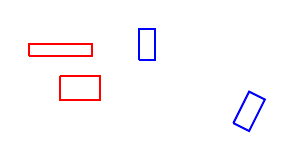
\begin{tikzpicture}
    \visible<3> {
    	% Sahel
    	\draw[red, line width = 0.25mm] (3.2,5.25) -- (4.0,5.25) -- (4.0,5.4) -- (3.2,5.4) -- (3.2,5.25);
    	
    	\draw[red, line width = 0.25mm] (3.6,5.0) -- (4.1,5.0) -- (4.1,4.7) -- (3.6,4.7) -- (3.6,5.0);
    }
	 \visible<4> {
	 	\draw[blue, line width = 0.25mm] (4.6,5.2) -- (4.8,5.2) -- (4.8,5.6) -- (4.6,5.6) -- (4.6,5.2);
	 	
	 	\draw[blue, line width = 0.25mm] (5.8,4.4) -- (6.0,4.3) -- (6.2,4.7) -- (6.0,4.8) -- (5.8,4.4);
	 }
	\end{tikzpicture}
	\end{textblock*}
	\begin{textblock*}{14cm}(6.7cm,1.45cm)
		\only<3->{
		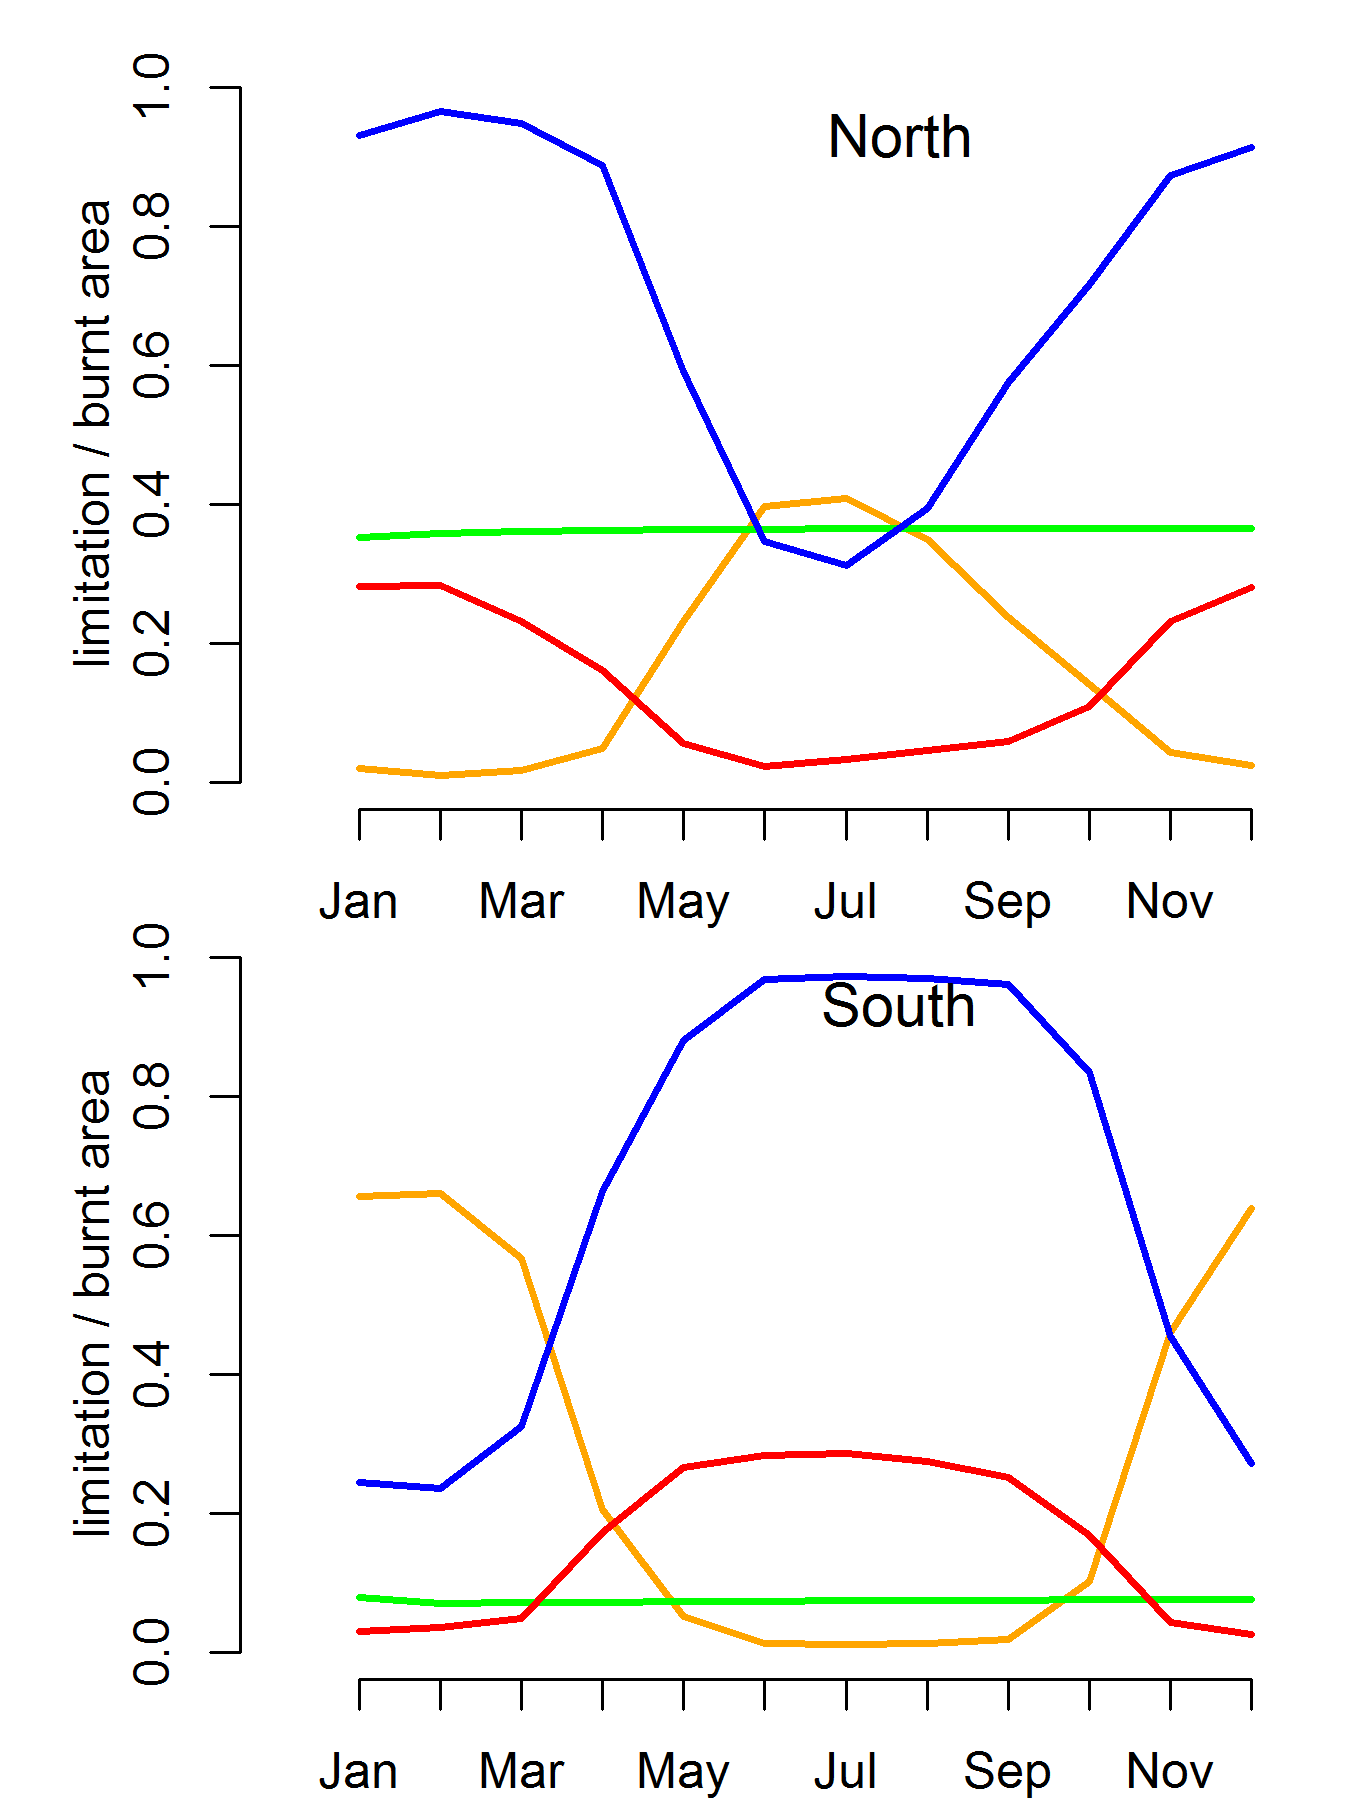
\includegraphics[width=5.7cm]{images/caseStudy/seasonal_casestudyAfrica}}
		\only<4->{
			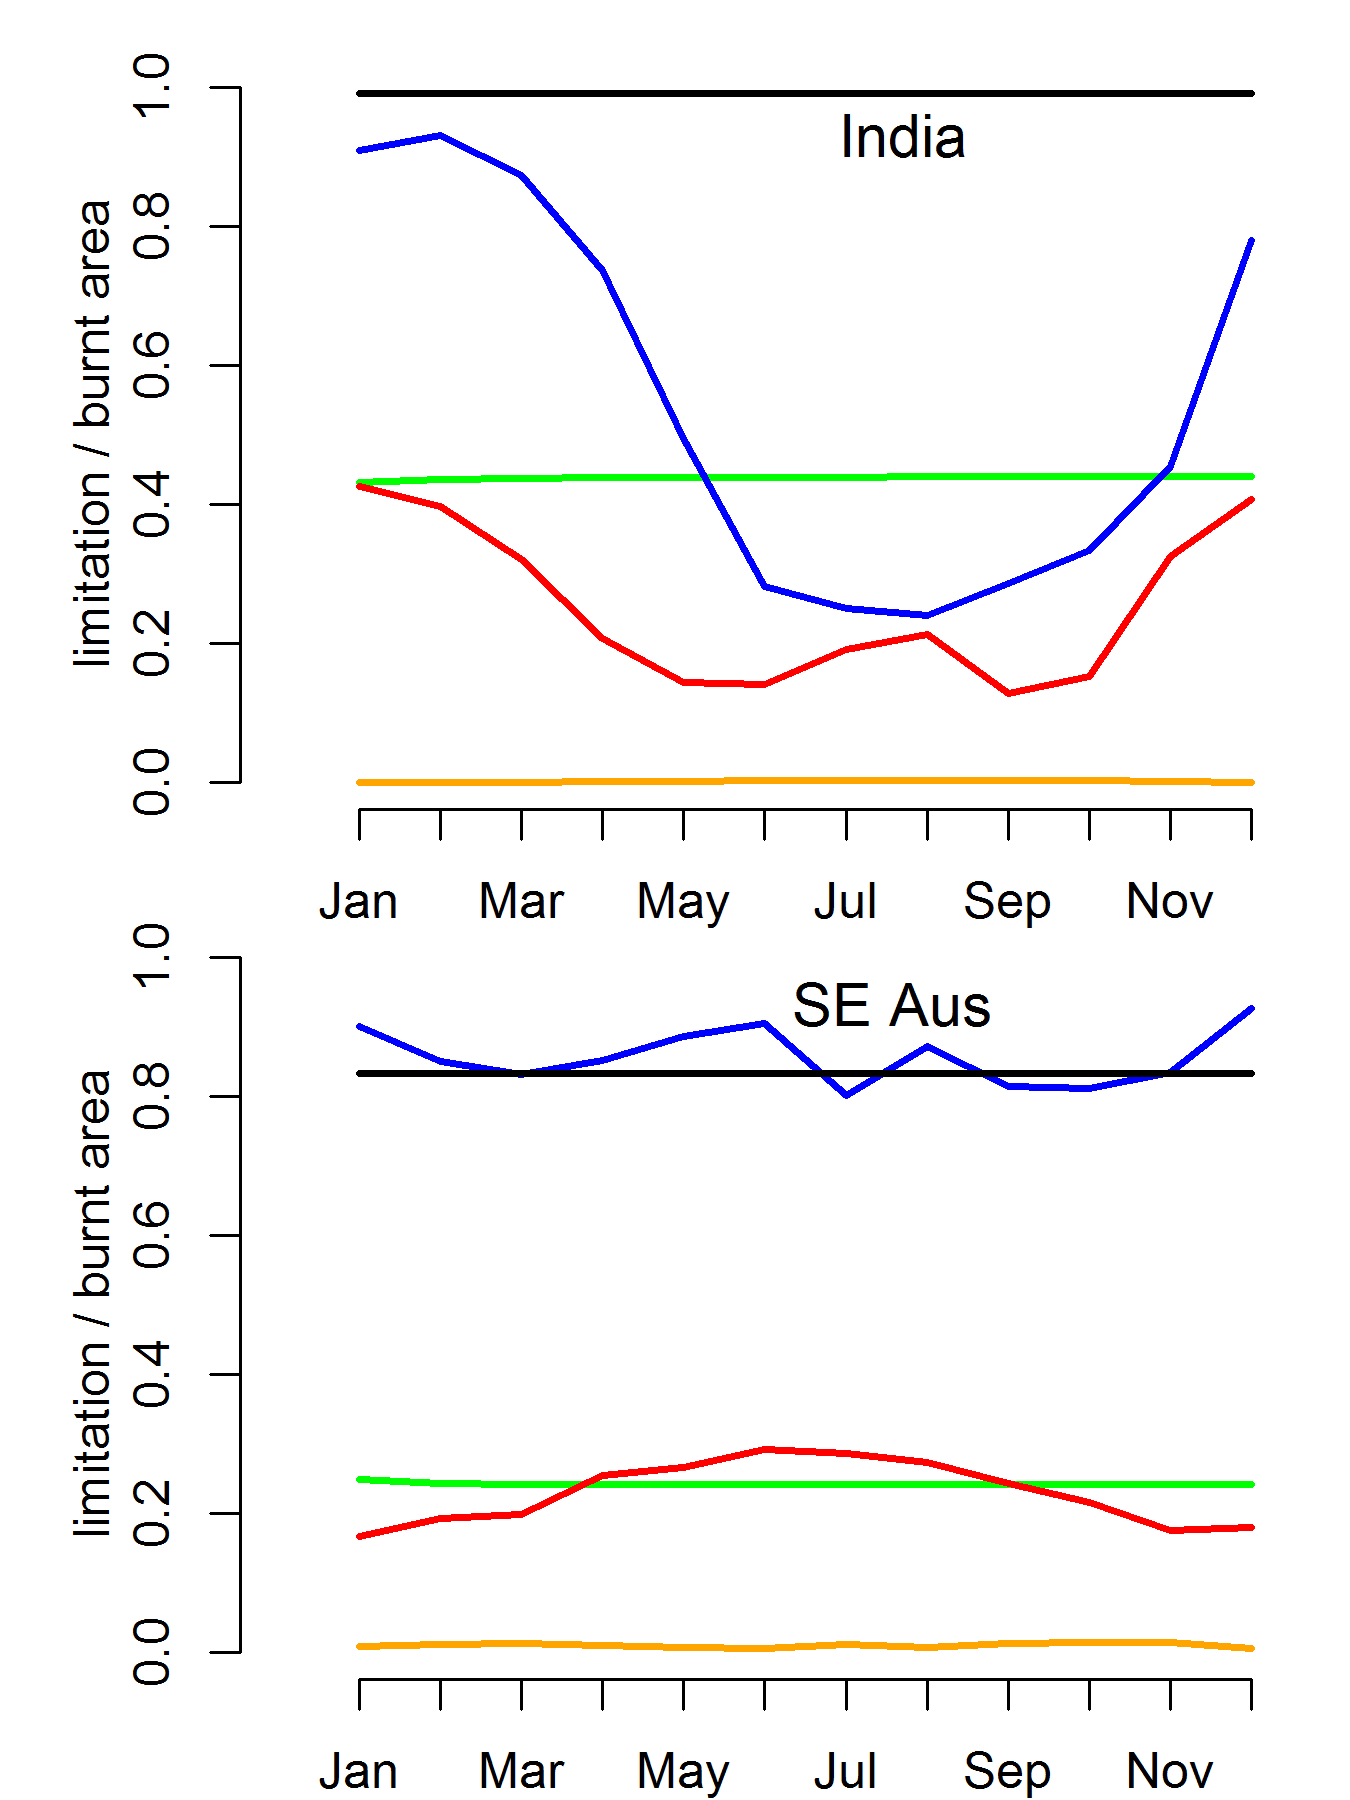
\includegraphics[width=5.7cm]{images/caseStudy/seasonal_casestudyAsia1}}
	\end{textblock*}
\end{frame}

%\section{Results}\label{results}
In this section we describe the results.

%\subsection{Benchmarking}

\begin{figure}[!ht]
  \centering
    \includegraphics[width=0.67\textwidth]{../figs/gfedComparison.png}
  \caption{Benchmark comparisons against GFED4s \citep{Giglio2013}.}
\end{figure}

%\subsection{Limitations}

\begin{figure}[!ht]
  \centering
    \includegraphics[width=0.67\textwidth]{../figs/limitation_lines.png}

  \caption{Limitation contribution for each control.}
\end{figure}


%\subsection{Sensitivity}

\begin{figure}[!ht]
  \centering
    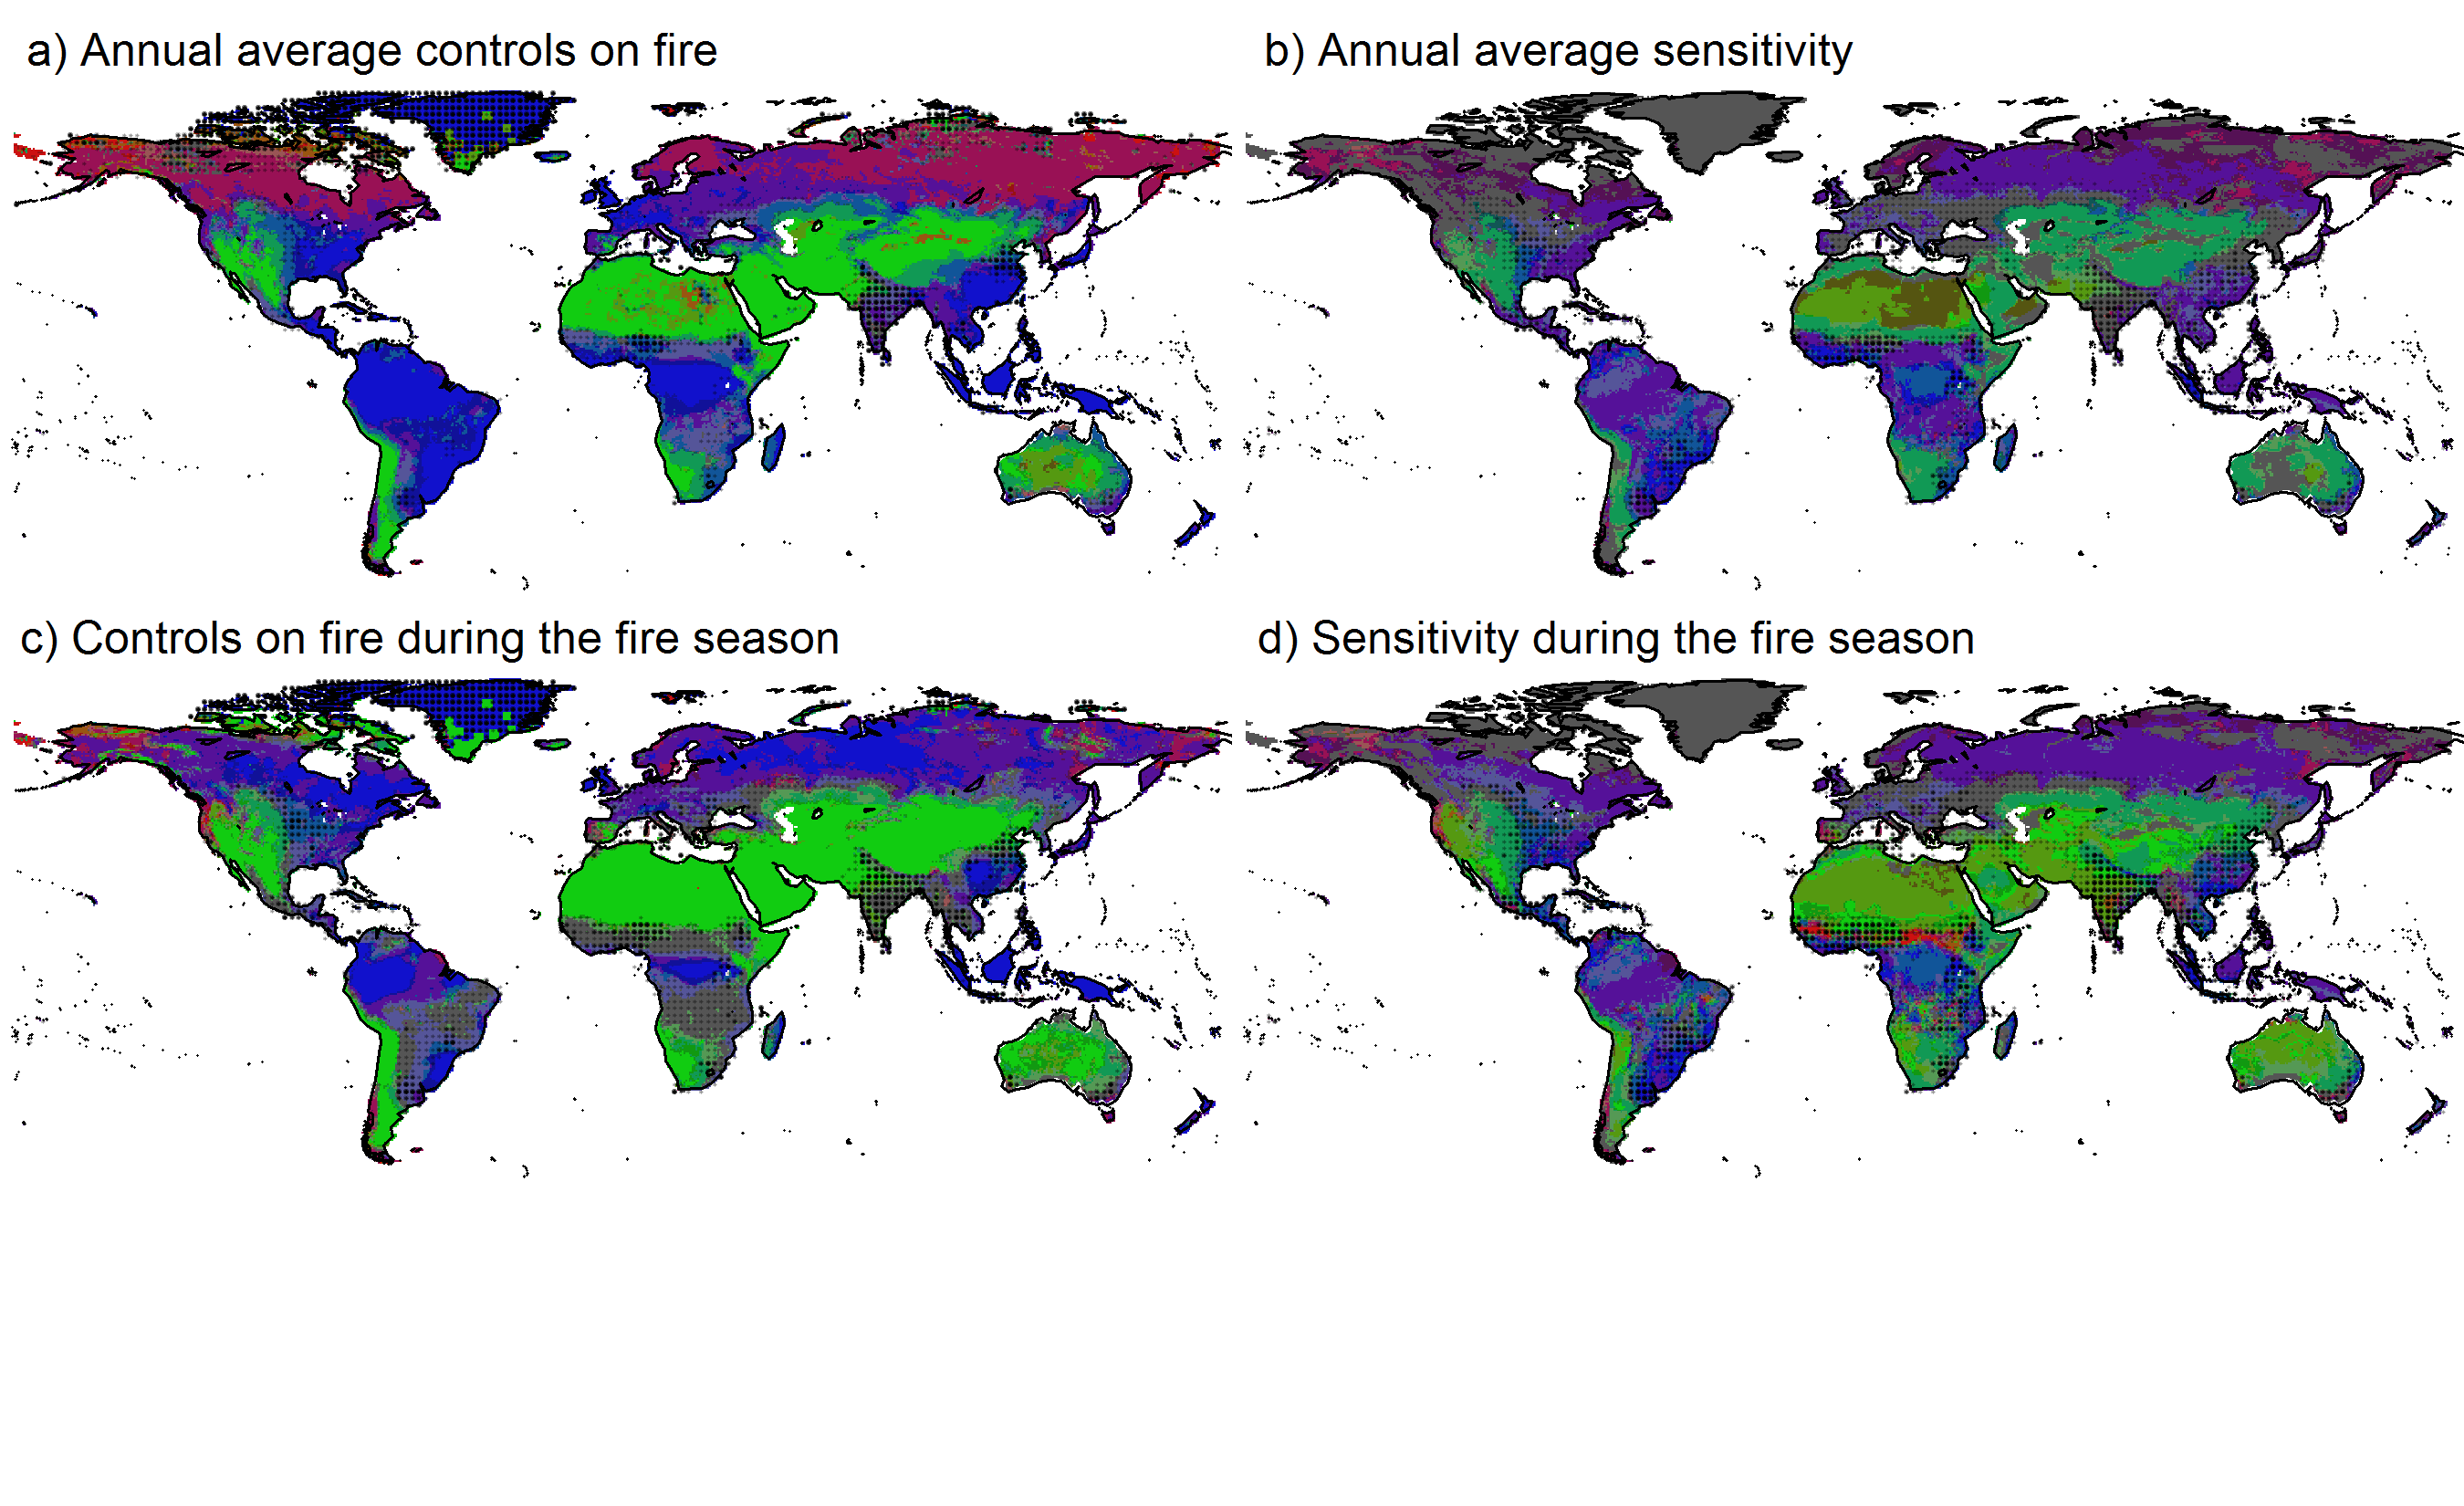
\includegraphics[width=0.67\textwidth]{../figs/limitation_map.png}

  \caption{Limitation and sensitivity.}
\end{figure}

\begin{figure}[!ht]
  \centering
    \includegraphics[width=0.67\textwidth]{../figs/moisture_change_for_Amazon_tipping_point.png}

  \caption{Required change in \% fuel moisture content to induce savanna-level fire in the Amazon.}
\end{figure}


%\subsection{Human impact}

\begin{figure}[!ht]
  \centering
    \includegraphics[width=0.67\textwidth]{../figs/HumanImpactMap_small.png}

  \caption{Human impact on burnt area.
            a) Increases in burnt area from human induced fire starts.
            b) Changes in burnt area from human fire starts and supression.}
\end{figure}

\begin{figure}[!ht]
  \centering
    \includegraphics[width=0.67\textwidth]{../figs/aguplot_Kelleyetal.png}

  \caption{AGU plot.}
\end{figure}


\begin{figure}[!ht]
  \centering
    \includegraphics[width=0.67\textwidth]{../figs/cropland_noCrop_impact.png}

  \caption{The impact of cropland on burnt area in non-cropland within the same gridcell.}
\end{figure}

%\section{Conclusions}\label{conclusions}

%\section{Papers and Applications}

\subsection{What limits fire, where and when: sensitivity of burnt area to different controls}

\subsubsection{Abstract}
Global fire models typically describe fire as a consequence of fuel load, moisture, natural and anthropogenic
ignitions, and land use suppression. A lack of information on the temporal and spatial distribution of these
controls has meant that their simulated effects on predicting burnt area are largely untested. Despite this,
there is a pervasive assumption that burnt area is proportional to the number of ignitions, with many models
predicting significant increases in burnt area with human fire starts.


Here, we map the limitation and sensitivity of burnt area to each control using a simple framework whereby
limitations are imposed by: fuel discontinuity; fuel moisture and atmospheric drying potential; lightning and
human ignitions; and land use. Limitations are described from remote sensed and meteorological
observations and optimized against Global Fire Emissions Database (GFED4s) burnt area observations.
Fuel moisture is shown to be the main limitation of fire over much of the world, (44\% annual average and
36\% during local dry seasons), particularly in the humid forests and cold, slow drying boreal areas. Fuel
discontinuity is the next limitation (25\% annually and 23\% in the dry season), especially in deserts and dry
season grasslands. This is followed by land use change (18\% annually, 21\% dry season) and then ignitions
(13\% annually, 19\% dry season), which is only a significant limiting factor in dry season savanna, where
rapid drying of fuel built up during the wet season removes all other natural limitations. In these areas,
changes in burnt area are actually more sensitive to other controls, typically land use.


This study contradicts the way basic processes are represented in many global fire models. As ignitions only
impact burnt area over a limited geographic extent, better representation of controls imposed by fuel loads
and moisture is vital. Human ignitions only contribute to a small increase in global burnt area (2\%), which is
offset by the dramatic impact of suppression through anthropogenic land cover changes. The assumption
that humans cause burnt area over much of the world is therefore clearly incorrect, and adequate simulation
of suppression through land use should become a priority. This result also has implications when considering
ecosystem services of agricultural land and fire management policies.

\pagebreak
x
\pagebreak
\subsection{Anthropagenic regime shifts}
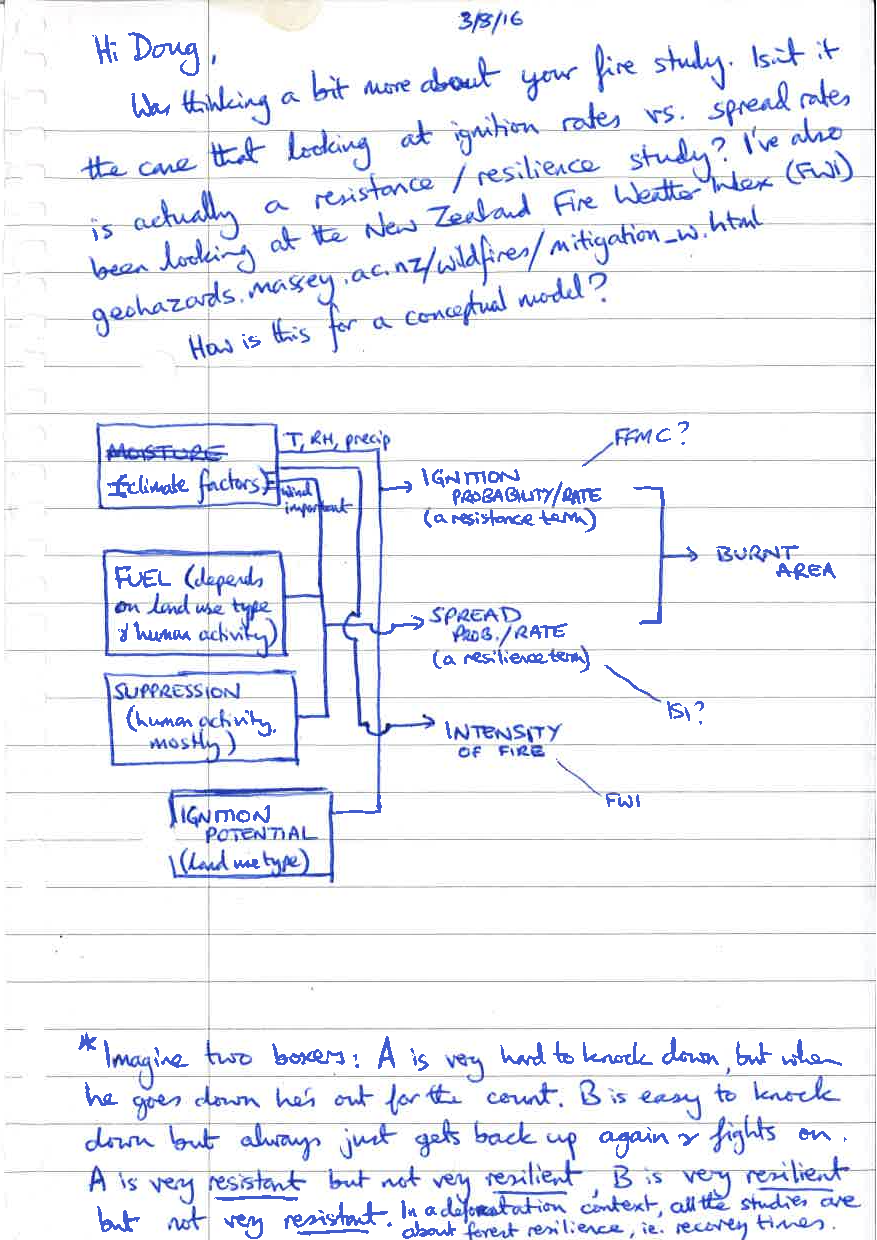
\includegraphics[width=0.99\textwidth]{diagrams/tobys_notes.pdf}


\pagebreak
\bibliographystyle{plainnat}
\bibliography{Model_description}

\end{document}
This is never printed
